\documentclass[a4paper14pt]{article}
\usepackage[english,russian]{babel}
\usepackage{graphicx} 
\usepackage{indentfirst}
\usepackage[left=25mm,right=15mm,top=40mm,bottom=20mm]{geometry}
\usepackage{listings}
\usepackage{color}
\usepackage{setspace}
\onehalfspacing
\definecolor{mygreen}{rgb}{0,0.6,0}
\definecolor{mygray}{rgb}{0.5,0.5,0.5}
\definecolor{mymauve}{rgb}{0.58,0,0.82}
 
\lstset{ %
  backgroundcolor=\color{white},   % choose the background color; you must add \usepackage{color} or \usepackage{xcolor}
  basicstyle=\footnotesize,        % the size of the fonts that are used for the code
  breakatwhitespace=false,         % sets if automatic breaks should only happen at whitespace
  breaklines=true,                 % sets automatic line breaking
  captionpos=b,                    % sets the caption-position to bottom
  commentstyle=\color{mygreen},    % comment style
  deletekeywords={...},            % if you want to delete keywords from the given language
  escapeinside={\%*}{*)},          % if you want to add LaTeX within your code
  extendedchars=true,              % lets you use non-ASCII characters; for 8-bits encodings only, does not work with UTF-8
  frame=single,                    % adds a frame around the code
  keepspaces=true,                 % keeps spaces in text, useful for keeping indentation of code (possibly needs columns=flexible)
  keywordstyle=\color{blue},       % keyword style
  language=Octave,                 % the language of the code
  otherkeywords={*,...},           % if you want to add more keywords to the set
  numbers=left,                    % where to put the line-numbers; possible values are (none, left, right)
  numbersep=5pt,                   % how far the line-numbers are from the code
  numberstyle=\tiny\color{mygray}, % the style that is used for the line-numbers
  rulecolor=\color{black},         % if not set, the frame-color may be changed on line-breaks within not-black text (e.g. comments (green here))
  showspaces=false,                % show spaces everywhere adding particular underscores; it overrides 'showstringspaces'
  showstringspaces=false,          % underline spaces within strings only
  showtabs=false,                  % show tabs within strings adding particular underscores
  stepnumber=2,                    % the step between two line-numbers. If it's 1, each line will be numbered
  stringstyle=\color{mymauve},     % string literal style
  tabsize=2,                       % sets default tabsize to 2 spaces
  title=\lstname                   % show the filename of files included with \lstinputlisting; also try caption instead of title
}

\addtolength{\topmargin}{-3cm}
\addtolength{\textheight}{3cm}
\begin{document}
\newpage
\setcounter{page}{3}
\tableofcontents
\newpage
\section{Введениe}
Передача информации – это физический процесс, посредством которого осуществляется перемещение зна- ков (сведений, способных предоставлять информацию) в пространстве или осуществляется физический до- ступ субъектов к знакам. В общем случае возможно распространение самых различных видов сообщений: текстов, изображений, музыки, видео и др. Совокупность средств, служащих для передачи информации, называется системой передачи информации.\\
\indent В современных сетях связи используются аналоговые и цифровые системы передачи информации с тенденцией постепенного перехода к применению только цифровых систем. Однако в ближайшем будущем большое число соединений будет устанавливаться с использованием обеих технологий. Для обеспечения в этих условиях заданных характеристик каналов и трактов, гарантирующих высокое качество передачи информации, принципы проектирования цифровых и аналоговых систем передачи должны быть совместимы.\\
\indentДля повышения достоверности передачи данных, представления их в удобной форме, обеспечения ми- нимума среднего числа символов на одно сообщение информация преобразуется с помощью кодирующего устройства. Сообщения представляют собой либо последовательность импульсов, означающую линейный код (в полосе пропускания), либо ограничивается набором непрерывно меняющейся формы волны, используя метод цифровой модуляции. Модуляция и соответствующая ей демодуляция осуществляются модемным оборудованием.\\
\indentИнформация в кабельных сетях передается в закодированном виде, то есть каждому биту передаваемой информации соответствует свой набор уровней электрических сигналов в сетевом кабеле. Передача происходит без модуляции или, как еще говорят, в основной полосе частот. Модуляция высокочастотных сигналов применяется в основном в бескабельных сетях, в радиоканалах.\\
\indentЦелями работы являются изучение и анализ линейного кода NRZ, разработка и описание программы для кодирования и декодирования данных, обзор преимуществ и недостатков метода. Также будет проведено тестирование программной реализации с целью проверки корректности её работы.\\
\newpage
\section{Теоретическая часть}
\subsection{Общие понятия о кодировании}
Кодированием называется процесс преобразования сообщения в комбинации из дискретных сигналов. Оно применяется для минимизации объёма передаваемых данных, повышения ее достоверности, увеличения скорости передачи, а также повы- шения помехоустойчивости путём внесения дополнительной избыточности. Правильный выбор кода позволяет снизить требования к выбору кабеля. Например, при разных кодах предельная скорость передачи по одному и тому же кабелю может отличаться в два раза. Код должен в идеале обеспечивать хорошую синхронизацию приема, низкий уровень ошибок, работу с любой длиной передаваемых информационных последовательностей. Код также влияет на сложность сетевой аппаратуры, а именно на узлы кодирования и декодирования.\\ 
\indentЛинейным кодированием называется процесс преобразования информации, представленной в цифровом виде, то есть хранящейся в формате серии из нулей и единиц, в цифровой сигнал.\\
\indentПри линейном кодировании передача большего количества битов выполняется в одном сигнале, благодаря чему используемая ширина полосы значительно уменьшается. Мощность пропускания данной полосы используется наиболее эффективно, плотность мощности очень благоприятная. Содержание времени является адекватным. При линейном кодировании избегают длинных строк 1 и 0, что позволяет сохранить прозрачность. Вероятность ошибки значительно снижается.\\
\indentРазличают 3 типа линейного кодирования: однополярный, полярный и биполярный 
Однополярная сигнализация также называется включением-выключением, или просто OOK. Наличие импульса представляет собой 1, а отсутствие импульса представляет собой 0.\\
\indentВ полярном типе передачи сигналов максимум данных представлен положительным импульсом, а минимум данных представлен отрицательным импульсом.\\
\indentМетод биполярного кодирования предполагает наличие трех уровней напряжения, а именно +, – и 0. Такой сигнал называется двойным двоичным сигналом.\\
Данные типы сигнализация реализуются за счет применения кода NRZ («Невозврат к нолю») или RZ («Возврат к нулю»).\\
\indentВ зависимости от количества уровней напряжения, используемых для формирования сигналов чаще всего встречаются следующие виды систем линейного кодирования:\\
\begin{itemize}
    \item[-]Двухуровневое кодирование
    \item[-]Трёхуровневое кодирование
    \item[-]Четырёхуровневое кодирование
    \item[-]Многоуровневое кодирование
\end{itemize}
\newpage
\begin{figure}[h]
    \center{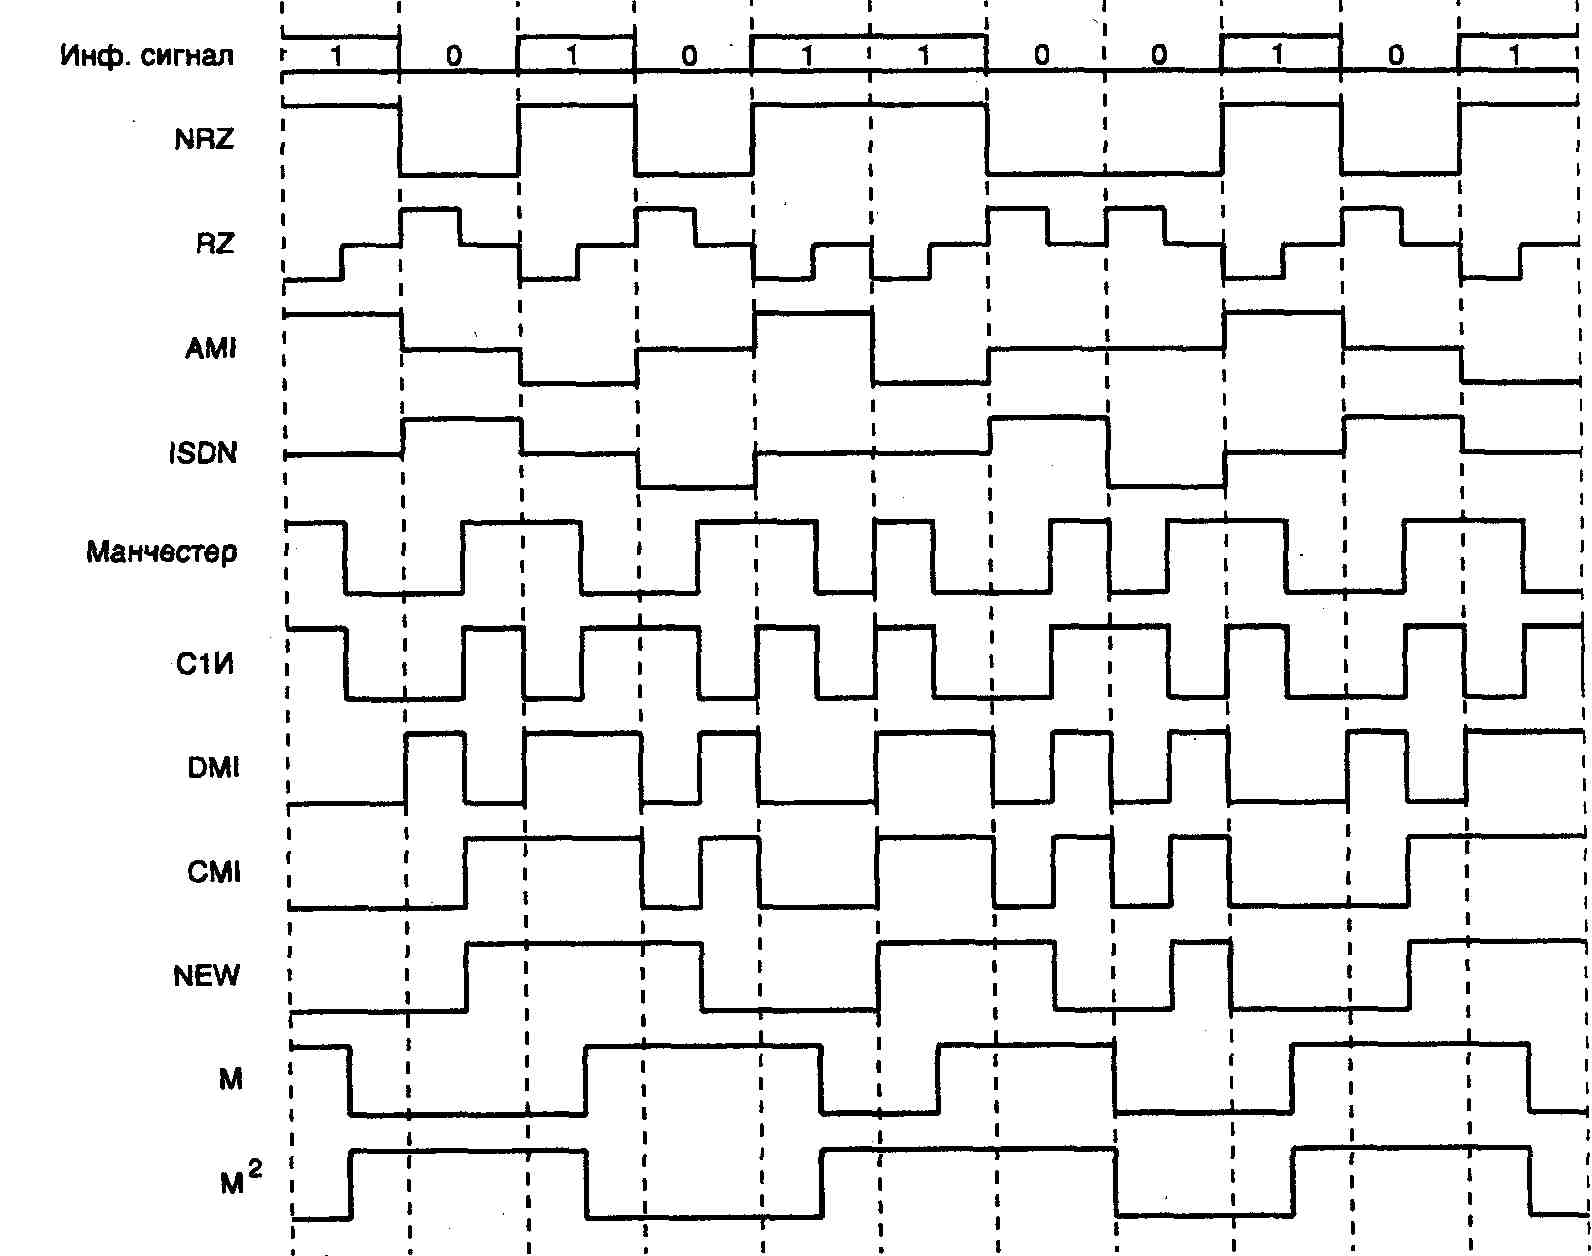
\includegraphics[width=0.8\textwidth]{examples.jpg}}
    \caption{Примеры линейного кодирования}
\end{figure}
\\
    Одним из видов линейного кодирования является код NRZ.
\newpage
\subsection{Описание кода NRZ}
\indentКод NRZ (non return to zero) — один из способов линейного кодирования, используется при передаче дискретных сообщений в канале связи, формируя сигнал, передаваемый на расстояние.\\
\indentПри передаче информации на расстояние информация представляется в цифровом виде и в канал связи формируется сигнал в соответствии с кодом: логическому нулю соответствует нижний уровень сигнала, логической единице соответствует верхний уровень сигнала.\\
\indent NRZ-код не является самосинхронизирующимся, поэтому в устройствах передачи данных для синхронизации сигнала применяют скремблирование — в последовательность специально вводят детерминированный процесс, по которому происходит синхронизация тактовой частоты приёмника с передатчиком.\\
\indentВ спектре сигнала присутствует низкочастотная составляющая, которая приближается к постоянному сигналу при передаче серии передаваемых последовательностей из логических «единиц» или «нулей».\\
\subsection{Варианты представления кода NRZ}
Различают несколько вариантов представления кода:
\begin{itemize}
    \item[-]Униполярный код — логическая единица представлена верхним потенциалом, логический нуль представлен нулевым потенциалом;    
    \item[-]Биполярный код — логическая единица представлена положительным потенциалом, логический нуль представлен отрицательным потенциалом.
\end{itemize}
\begin{figure}[h]
    \center{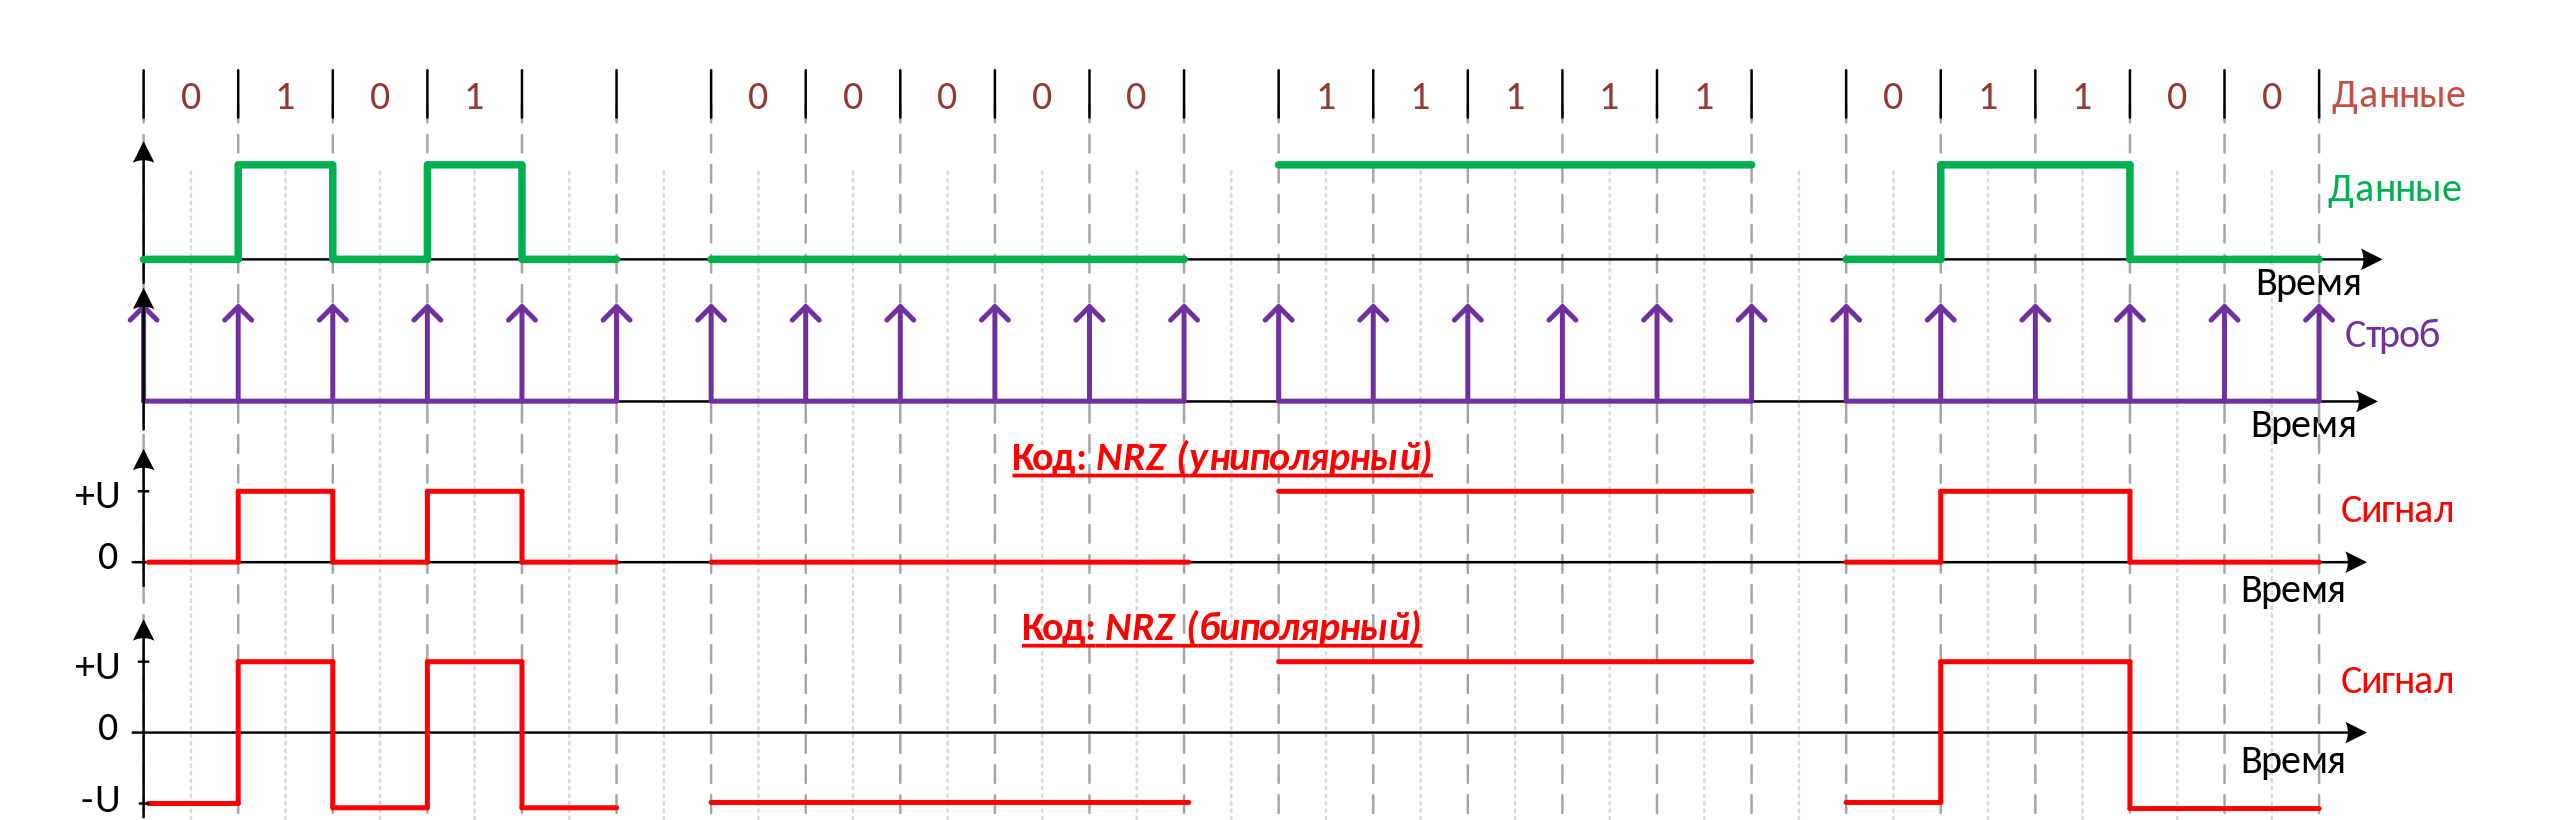
\includegraphics[width=0.9\textwidth]{nrz.png}}
    \caption{Пример NRZ кодирования}
\end{figure}
\newpage
\subsection{Достоинства}
\begin{itemize}
    \item Простота реализации кода — код полностью соответствует поступающей на вход передатчика битовой последовательности и никаких дополнительных преобразований выполнять не нужно; 
    \item Минимальная необходимая полоса пропускания линии связи. 
\end{itemize}
\subsection{Недостатки}
\begin{itemize}
    \item Потеря синхронизации во время приема слишком длинных блоков (пакетов) информации. В связи с этим код NRZ используется только для передачи короткими пакетами (обычно до 1 Кбита);
    \item Код может обеспечить обмен сообщениями (последовательностями, пакетами) только фиксированной, заранее обговоренной длины, поскольку по принимаемой информации приемник не может определить, идет ли еще передача или уже закончилась;
    \item Необходимость передачи старт-стопового бита для синхронизации приёмника с передатчиком;
    \item Наличие постоянной составляющей (ёмкостное сопротивление), из-за чего невозможно обеспечить гальваническую развязку с помощью трансформатора;
    \item Наличие ёмкостного сопротивления (в униполярном коде) — нарастание в проводном канале связи постоянной составляющей (паразитной ёмкости), которое препятствует функциональности электрооборудования (проблема решается за счет использования биполярного кода);
    \item Нарушение плотности следования единичных импульсов (плохая синхронизация приёмника и передатчика) — при передаче последовательности логических нулей или единиц происходит рассинхронизация передатчика и приемника;
    \item Для синхронизации передатчика с приемником применяется избыточность передачи данных (вводятся детерминированные последовательности, по которым производится синхронизация) или скремблирование, что усложняет реализацию и уменьшает скорость передачи данных.
\end{itemize}
\subsection{Сравнение кодов NRZ и RZ}
Код RZ (return to zero – с возвратом к нулю) – это трехуровневый код, который принципиально отличаются от NRZ тем, что сигнал имеет дополнительные переходы, используемые для синхронизации. В центре битового интервала всегда есть переход сигнала (положительный или отрицательный), следовательно, из этого кода приемник легко может выделить синхроимпульс (строб). Возможна временная привязка не только к началу пакета, как в случае кода NRZ, но и к каждому отдельному биту.\\
\indentЕще одно важное достоинство кода RZ – простая временная привязка приема, как к началу последовательности, так и к ее концу. Приемник просто должен анализировать наличие изменения уровня сигнала в течение битового интервала. Первый битовый интервал без изменения уровня сигнала соответствует окончанию принимаемой последовательности бит. Поэтому в коде RZ можно использовать передачу последовательностями переменной длины.\\
\indentЗначимый недостаток кода RZ состоит в том, что для него требуется вдвое большая полоса пропускания канала при той же скорости передачи по сравнению с NRZ (так как здесь на один битовый интервал приходится два изменения уровня сигнала). Другой важный недостаток – наличие трех уровней, что всегда усложняет аппаратуру как передатчика, так и приемника.\\
\indentКод RZ применяется не только в сетях на основе электрического кабеля, но и в оптоволоконных сетях. \\
\begin{figure}[h]
    \center{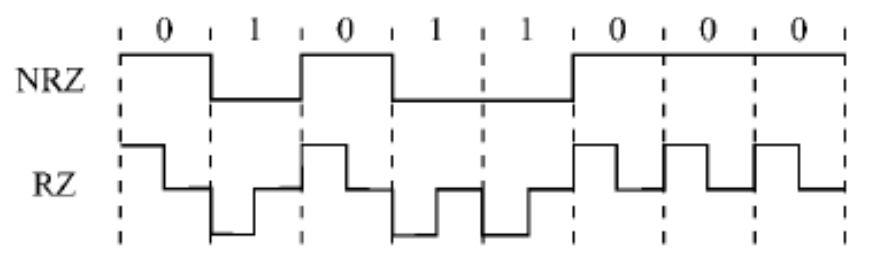
\includegraphics[width=0.9\textwidth]{rzvsnrz.jpg}}
    \caption{Сравнение кодов NRZ и RZ}
\end{figure}
\subsection{Применение}
Наиболее известное применение кода NRZ – это стандарт RS232-C, последовательный порт персонального компьютера. Передача информации в нем ведется байтами (8 бит), сопровождаемыми стартовым и стоповым битами.

\newpage

\section{Аналитическая часть}
Цели исследования:
\begin{itemize}
    \item[-]Выбор и анализ алгоритмов кодера и декодера;
    \item[-]Разработка и описание программной реализации кодера и декодера;
    \item[-]Проверка корректности работы разработанного варианта
программной реализации системы передачи информации.
\end{itemize}
Предполагается, что кодер на основе кода NRZ преобразует входные данные в закодированную последовательность. Декодер выполняет обратную операцию. Пользователь сможет получать результат в формате закодированных и декодированных комбинаций в виде списка, а также осциллограмм.\\
\indentВ качестве среды для разработки выбрано окружение ОС Ubuntu 10.3.0 x64, язык программирования Python3 с модулем графики matplotlib.

\newpage
\section{Практическая часть}
\subsection{Структура программы}
Программная реализация кодера и декодера состоит из модуля rz.py, в Приложении 1 приведен листинг. Данный модуль содержит необходимые функции для кодирования и декодирования данных.\\
\indentФункции, реализованные в кодере, позволяют преобразовывать комбинацию из нулей и единиц в закодированную последовательность, а также позволяют выводить результат на экран в виде осциллограммы.\\
\indentФункции декодера формируют декодированную последовательность из закодированных данных и позволяют выводить результат на экран в виде осциллограммы.\\
\indentДалее опишем функции, которые используются как в кодере, так и в декодере.\\
\subsection{Программная реализация кодера}
\indent Программа принимает в качестве параметра последовательность из нулей и единиц и, используя правила преобразования в коде NRZ, возвращает закодированные данные в виде списка.\\
\indentПеред кодированием информации проверяется, инициализирован ли переданный функции список. Если последовательность содержит None, то вызывается исключение.\\
\indentЕсли список инициализирован, то дальше вычисляется его длина. В случае, когда длина последовательности равна нулю, то есть он не содержит каких-либо данных, срабатывает исключение.\\
\indentСоздаётся новый список, в который мы будем записывать закодированные данные. После этого в цикле происходит последовательное преобразование исходной комбинации. Передаваемый в качестве аргумента список должен содержать только нули или единицы. При обнаружении каких-либо других значений вызывается исключение.\\
\indentЕсли очередной элемент списка равен единице, то в список записывается 1, что соответствует отрицательному уровню напряжения. Иначе в закодированный список помещается 0.\\

\begin{figure}[h!]
    \center{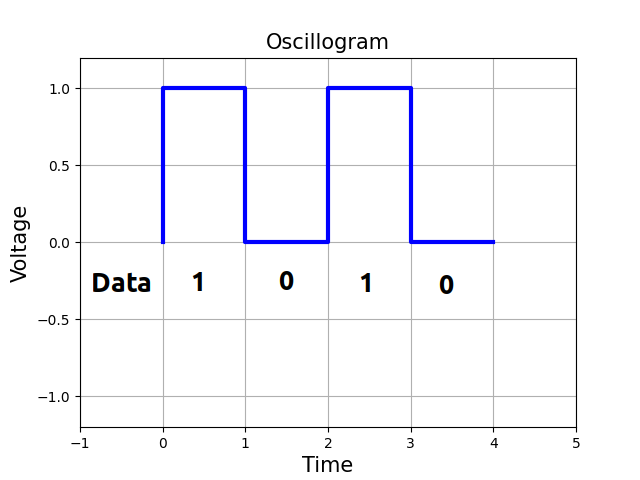
\includegraphics[width=0.9\textwidth]{1010.png}}
    \caption{Изображение участка закодированного сигнала}
\end{figure}

\indentНа рисунке изображен участок сигнала, закодированной последовательности кодом NRZ.

\newpage
\subsection{Программная реализация декодера}
\indentПрограмма принимает в качестве параметра последовательность из 0 и 1 и, согласно правилам преобразования в коде NRZ, возвращает декодированную серию из нулей и единиц в виде списка. Перед декодированием информации проверяется, инициализирован ли переданный функции список. Если последовательность содержит None, то вызывается исключение.\\
\indentЕсли список создан, то далее вычисляется его длина. В случае, когда длина списка равна нулю, то есть он не содержит каких-либо данных, срабатывает исключение.\\
\indentСоздаётся новый список декодированной последовательности в который мы будем добавлять декодированные данные. После этого в цикле происходит последовательное преобразование закодированной последовательности. Передаваемый в качестве аргумента список должен содержать только 0 и 1. В случае обнаружения каких-либо других значений вызывается исключение.\\
\indentФункция возвращает список с декодированными данными.\\
\begin{figure}[h!]
    \center{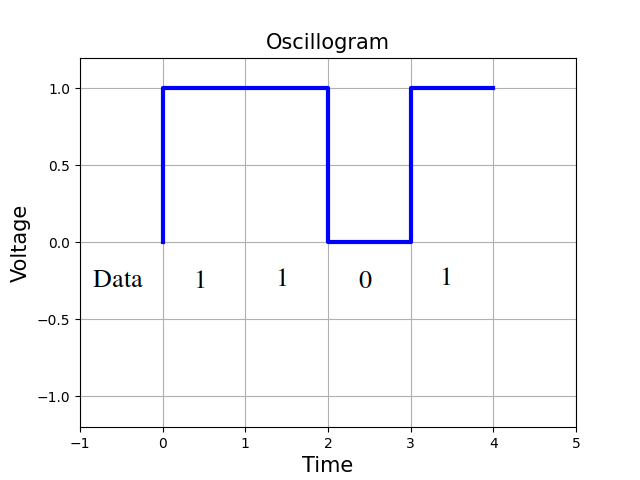
\includegraphics[width=0.9\textwidth]{1101.png}}
    \caption{Изображение участка декодированного сигнала}
\end{figure}

\indentНа рисунке изображен участок сигнала, декодированной последовательности кода NRZ.\\
\newpage
\subsection{Пример кодирования}
\indentПродемонстрируем пример работы кодера. Сначала получим закодированную последовательность в виде списка и выведем результат в консоль.\\
\noindentИсходные данные:\\ 
\indent[1, 0, 1, 0, 1, 1, 0, 0].\\
\newpage
\noindentВоспользуемся программой coder\_example1.py.\\

\begin{figure}[h!]
    \center{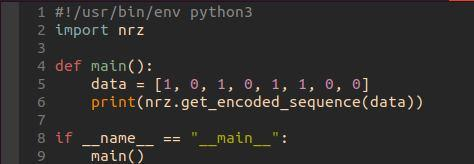
\includegraphics[width=0.6\textwidth]{example11.jpg}}
    \caption{Код программы coder\_example1.py}
\end{figure}

\noindentПри запуске программы получим результат:\\
\begin{figure}[h!]
    \center{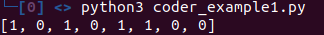
\includegraphics[width=0.6\textwidth]{console11.png}}
    \caption{Результат выполнения программы coder\_example1.py}
\end{figure}

\indentТеперь получим осциллограмму для той же последовательности при помощи программы coder\_example2.py.

\begin{figure}[h!]
    \center{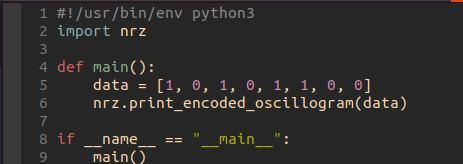
\includegraphics[width=0.6\textwidth]{example12.jpg}}
    \caption{Код программы coder\_example2.py}
\end{figure}

\newpage
Результат программы:

\begin{figure}[h]
    \center{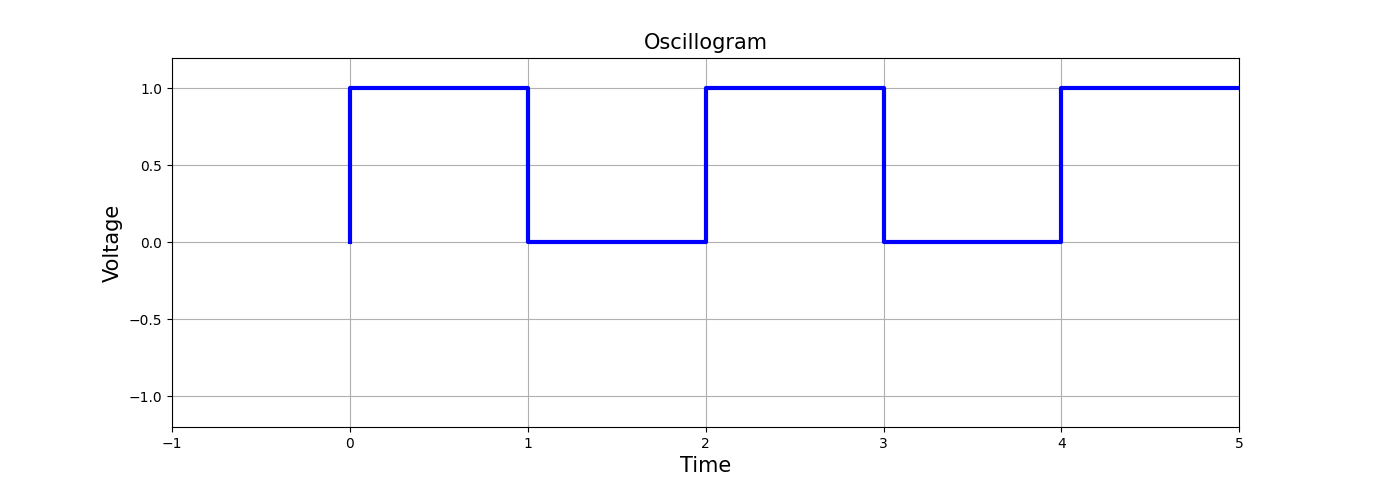
\includegraphics[width=0.6\textwidth]{osc1.png}}
    \caption{Результат выполнения программы coder\_example2.py}
\end{figure}
\subsection{Пример декодирования}
\indentПродемонстрируем пример работы декодера. Сначала получим декодированную последовательность в виде списка и выведем результат в консоль.\\
\noindentИсходные данные:\\ 
\indent [1, 0, 1, 0, 1, 0, 1, 0, 1, 0, 1, 0, 1, 0, 1, 0]\\
\noindentВоспользуемся программой coder\_example1.py.\\

\begin{figure}[h!]
    \center{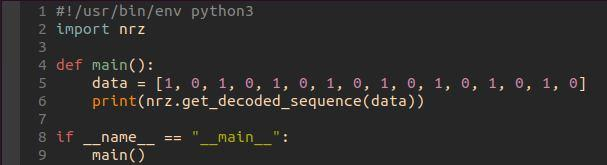
\includegraphics[width=0.6\textwidth]{example21.jpg}}
    \caption{Код программы decoder\_example1.py}
\end{figure}

\noindentПри запуске программы получим результат:\\

\begin{figure}[h!]
    \center{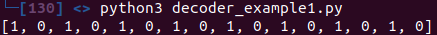
\includegraphics[width=0.6\textwidth]{console21.png}}
    \caption{Результат выполнения программы decoder\_example1.py}
\end{figure}

\indentТеперь получим осциллограмму для той же последовательности при помощи программы decoder\_example2.py.\\

\begin{figure}[h!]
    \center{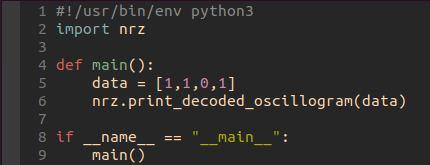
\includegraphics[width=0.6\textwidth]{example22.jpg}}
    \caption{Код программы decoder\_example2.py}
\end{figure}

Результат программы:\\

\begin{figure}[h!]
    \center{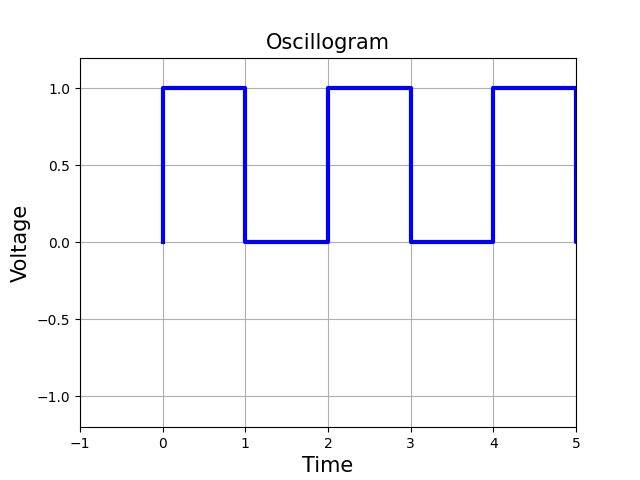
\includegraphics[width=0.6\textwidth]{osc2.png}}
    \caption{Результат выполнения программы decoder\_example2.py}
\end{figure}
\newpage
\section{Заключение}
\indentВ данной работе был изучен и проанализирован код NRZ, рассмотрены его особенности, преимущества и недостатки. Реализована программа для кодирования и декодирования информации.\\

\indentРазработанная программная реализация выполняет функции кодирования и декодирования корректно, что проверено тестированием, результаты которого также приведены.\\

\newpage
\section*{Приложение 1}
\noindentФайл nrz.py
\lstset{language=Python}
\begin{lstlisting}
#!/usr/bin/env python3
import matplotlib.pyplot as plt

def set_settings():
    plt.xlim([-1, 5])
    plt.ylim([-1.2, 1.2])
    plt.xlabel('Time', fontsize=15, color='black')
    plt.ylabel('Voltage', fontsize=15, color='black')
    plt.grid(True)
    plt.title("Oscillogram", fontsize=15)

def print_oscillogram(x_coordinates, y_coordinates):
    set_settings()
    plt.plot(x_coordinates, y_coordinates, 'b', linewidth=3)
    plt.show()

def print_encoded_oscillogram(sequence):
    y_coordinates = get_y_coordinates_for_encoding(get_encoded_sequence(sequence))
    x_coordinates = get_x_coordinates_for_encoding(len(y_coordinates))
    print_oscillogram(x_coordinates, y_coordinates)

def get_encoded_sequence(sequence):
    if sequence == None:
        raise Exception("Your sequence is None!")
    if len(sequence) == 0:
        raise Exception("The size of your sequence is zero!")

    encoded_sequence = []
    for i in range (len(sequence)):
        if sequence[i] != 0 and sequence[i] != 1:
            raise Exception("Incorrect data format!")
        if sequence[i] == 1:
            encoded_sequence.append(1)
        else:
            encoded_sequence.append(0)
    return encoded_sequence

def get_y_coordinates_for_encoding(sequence):
    y_coordinates = []
    y_coordinates.append(0)
    for i in range(0, len(sequence)):
        y_coordinates.append(sequence[i])
        y_coordinates.append(sequence[i])
    return y_coordinates

def get_x_coordinates_for_encoding(length):
    sequence = []
    step = 0
    sequence.append(step)
    for i in range(1, length, 4):
        sequence.append(step)
        step += 1
        sequence.append(step)
        sequence.append(step)
        step += 1
        sequence.append(step)
    return sequence

def print_decoded_oscillogram(sequence):
    y_coordinates = get_y_coordinates_for_decoding(get_decoded_sequence(sequence))
    x_coordinates = get_x_coordinates_for_decoding(len(y_coordinates))
    print_oscillogram(x_coordinates, y_coordinates)

def get_decoded_sequence(sequence):
    if sequence == None:
        raise Exception("Your sequence is None!")
    if len(sequence) == 0:
        raise Exception("The size of your sequence is zero!")
    decoded_sequence = []
    for i in range (len(sequence)):
        if sequence[i] != 0 and sequence[i] != 1:
            raise Exception("Incorrect data format!")
        if sequence[i] == 1:
            decoded_sequence.append(1)
        else:
            decoded_sequence.append(0)
    return decoded_sequence

def get_y_coordinates_for_decoding(sequence):
    y_coordinates = []
    y_coordinates.append(0)
    for i in range(0, len(sequence)):
        y_coordinates.append(sequence[i])
        y_coordinates.append(sequence[i])
    return y_coordinates

def get_x_coordinates_for_decoding(length):
    sequence = []
    step = 0
    sequence.append(step)
    for i in range(1, length, 2):
        sequence.append(step)
        step += 1
        sequence.append(step)
    return sequence
\end{lstlisting}
\end{document}
